The Generalized Singular Value Decomposition is powerful in solving many numerical linear algebra problems as well as problems in other disciplines, such as statistics and signal processing. We briefly introduce several prominent applications and highlight one application in genome analysis in this section.    

\subsection{Prominent applications of the GSVD}

\paragraph{Tikhonov regularization.}
Tikhonov regularization in general form can be analyzed with the truncated GSVD when we are to solve the ill-posed linear least squares problem. \cite{hansen1989regularization} \cite{dykes2014simplified} \cite{wei2016tikhonov} Computerized ionospheric tomography \cite{bhuyan2004application} is one of the applications in this regard. 

\paragraph{Matrix pencil $A - \lambda B$.}
The GSVD is also used in the field of the canonical structure of matrix pencil $A-\lambda B$. \cite{kaagstrom1984generalized} More specifically, the column and row nullities of $A$ and $B$ and common null space reveal the information about the Kronecker structure of $A-\lambda B$.

\paragraph{Generalized total least squares problem.}
By making use of the GSVD, one can solve the generalized TLS problem. TLS is also called error-in-variable regression in statistics domain. The great advantage of the GSVD is that it replaces these implicit transformation of data procedures by one, which is numerically reliable and can more easily handle (nearly) singular associated error covariance matrix. \cite{van1989analysis} \cite{bai1992csd}

\paragraph{Genome analysis.}
The GSVD is applicable for comparative analysis of genome-scale expression datasets of two different organisms \cite{alter2003generalized} and is further extended to tensor \cite{sankaranarayanan2015tensor}. We will elaborate the role of the GSVD in genomes in Section \ref{genome-app}.

\paragraph{Oriented energy and oriented signal-to-signal ratio.}
In the context of oriented energy, one of the concerns is to characterize the signal-to-signal ratio of two given sequences of $m$-vectors $\{a_k\}$, $\{b_k\}$, $k = 1,\cdots,n$ with associated $m$-by-$n$ matrices $A$ and $B$. \cite{de1988mathematical} In other words, we're primarily interested in how to separate the desired signal (for instance $\{a_k\}$) from the undesired one ($\{b_k\}$). More specifically, given that rank($B$) = $l$, the question transforms to find the optimal $l$-dimensional subspace where the desired signal sequence $\{a_k\}$ can be optimally distinguished from the corrupting sequence $\{b_k\}$.

%\subsection{Subspaces of the $U$ matrix}\cite{edelman2019gsvd}
%The $U$ matrix of the GSVD provides orthonormal bases for three mutually orthogonal subspaces that are powerful in many applications: 
%
%\begin{equation*}
%    U = \begin{bmatrix}
%        \makecell{U_{1} = \\ \text{orthogonal basis for} \\ \{Ax:Bx=0\}} & \makecell{U_{2} = \\ \text{completion to all of} \\ col(A)=\{Ax\}} & \makecell{U_{3} = \\ \text{orthonomal basis for} \\ col(A)^{\perp}}
%    \end{bmatrix}
%\end{equation*}
%The ``completion'' referred to in the above equation means that taken together, the columns of $U_1$ and $U_2$ form and orthonormal basis for $col(A)$.

\paragraph{Linear discriminant analysis.}
Howland and Park \cite{howland2003structure} \cite{kim2005dimension} applied the GSVD to discriminant analysis to overcome the limitation of nonsingular covariance matrices that are used to represent the scatter within and between clusted text data. 

\paragraph{One Way ANOVA (Analysis of variance).}
A commonly used statistics test is to decide whether a proposed clustering of a vector $v$ is justified. The test takes the average square component in the $U_2$ direction and divides it by the average square component in the $U_3$ direction. \cite{wikipedia_2020}

%\subsection{The Jacobi ensemble from random matrix theory is a GSVD}\cite{edelman2019gsvd}
%Classical random matrix theory centers are Hermite, Laguerre, and Jacobi ensembles. Historically, they are presented in eigenvalue format, but we have argued that the eigenvalue, SVD, GSVD formats, respectively, are mathematically more natural providing simpler derviations and clearer insights. 

\subsection{GSVD in genome analysis} \label{genome-app}
With the advance of modern genomic technologies, scientists and researchers are able to acquire a wide range of molecular biological data, such as DNA-sequence and mRNA-expression, on a genomic scale at ease. For instance, DNA microarray, invented by Patrick O. Brown \cite{schena1995quantitative}, is a collection of microscopic DNA spots attached to a solid surface. Scientists use DNA microarrays to measure the expression levels of large numbers of genes simultaneously or to genotype multiple regions of a genome. DNA microarrays can be used to detect DNA (as in comparative genomic hybridization), or detect RNA (most commonly as cDNA after reverse transcription) that may or may not be translated into proteins.

What's more exciting is that once these data is ready, we can apply comparative analysis to understand the universality and specialization of molecular biology mechanisms. Specifically, such analysis helps us to distinguish the similarity and dissimilarity among two or more large-scale data sets. To this end, a mathematical framework is needed to remove the barriers of transferring genetic sequencing results to understandable information. Fortunately, the GSVD fits this purpose well: 
\begin{enumerate}
\item Two data sets are column-matched but row-independent matrices, where rows are genes and columns are samples. They exactly match the type of the input matrix pair of the GSVD. 
\item The GSVD simultaneously reduce the two ``genes'' $\times$ ``samples'' spaces to two diagonalized ``samplelets'' $\times$ ``genelets'' spaces. The column space is shared by both datasets. We can interpret the generalized singular values as the significance in one data set relative to that in the other.
\end{enumerate}

\subsubsection{Mathematical framework: the GSVD}
The GSVD is the simultaneous linear transformation of the two expression data sets $A$ and $B$ from $m$-genes-by-$n$-samples and $p$-genes-by-$n$-samples spaces to two reduced $n$-genelets-by-$n$-samplelets spaces, where both $m \gg n$ and $p \gg n$. 
\begin{equation}
	A = UC\onebytwo{0}{R}Q^T, \quad B = VS\onebytwo{0}{R}Q^T
\end{equation}

Notably, we have
\begin{enumerate}
\item $C^T C $ = diag($\alpha_1^{2}, \cdots, \alpha_n^{2}$), 
$S^T S$ = diag($\beta_1^{2}, \cdots, \beta_n^{2}$).
\item $Q$ is an $n$-by-$n$ orthogonal matrix. The rows of $Q$ form a basis for this row (or gene) space, and are denoted genelets.
\end{enumerate}


We then define the antisymmetric angular distance between two data sets:
\begin{equation}\label{eq-angular}
	\theta_{i} = arctan(\alpha_{i}/\beta_{i}) - \pi/4, \ \ \ \text{for } 1 \leq i \leq n 
\end{equation}

It indicates the relative significance of the $i$-th genelet, i.e., its significance in the first data set relative to that in the second. The $\pi/4$ offset means that an angular distance of 0 indicates a genelet of equal significance in both data sets. The angular distances are arranged in decreasing order of significance in the first data set relative to the second such that $\pi/4 > \theta_{1} > \theta_{2} > \cdots > \theta_{n} > -\pi/4$.

\Red{The notion of antisymmetric angular distance answers the question we have in general: given two matrices with equal columns, how can we classify the basis vectors in the rows of $Q$ according to its source. Mathematically, if $Q_{i}^{T}$ denotes the $i$-th row of $Q$, then the total projection of both data sets onto the genelet $Q_{i}^{T}$ can be thought of as the vector sum of these two orthogonal vectors, $\overrightarrow{\gamma_{i}} = \overrightarrow{\alpha_{i}} + \overrightarrow{\beta_{i}}$. The angle between the total projection $\overrightarrow{\gamma_{i}}$ and that of the second data set $\overrightarrow{\beta_{i}}$, $\theta_{i}$ above, measures the extent to which the total projection $\overrightarrow{\gamma_{i}}$ lies in the direction of the projection of either data set, $\overrightarrow{\alpha_{i}}$ or $\overrightarrow{\beta_{i}}$, and quantifies the relative contribution of each data set to this total projection. \cite{alter2003generalized} (Appendix)}

\subsubsection{Experiment}

We now illustrate this framework with the comparison between yeast and human cell cycle-expression data sets. \cite{tavazoie1999systematic} We also present experimental results, implemented in Julia. 

%\paragraph{Why yeast?} 
%The reasons of using yeast are two-fold. First, yeast cells share many basic biological properties with our cells. At least 20 per cent of human genes known to have a role in disease have counterparts in yeast. This suggests that such diseases result from the disruption of very basic cellular processes. Hence, yeast is also used to test new drugs. One may be surprised that antibiotic of penicillin is the first of its kind to be made by the yeast Saccharomyces cerevisiae. Second, genetic manipulation in yeast is easy and cheap compared to similar experiments in more complex animals such as mice and zebrafish.

\paragraph{Input data sets}
In our experiment, a single microarray probes the relative expression levels of $4523$ genes of yeast in a single sample. A series of $18$ arrays probes the genome-scale expression levels in $18$ different samples, i.e., under $18$ different experimental conditions. Similarly. Another set of microarrays probe the relative expression levels of $12056$ genes of human under $18$ experimental conditions. 

In other words, we have the following two matrices as inputs.
\begin{enumerate}
	\item $A$: a $4523$-by-$18$ matrix representing yeast cell expression
	\item $B$: a $12056$-by-$18$ matrix representing human cell expression
\end{enumerate}

\paragraph{Data pre-processing}
Unfortunately, microarray might fail to record gene expression in some samples. In other words, missing data might tabulate into some portion of the data set. In our experiment, 1825 out of 4523 rows have NULL entries for matrix $A$ and 7696 out of 12056 rows contain invalid entries in matrix $B$. 

One of the methods to impute missing data for genomic expressions is to utilize SVD to approximate the expression of all genes in the data set. \cite{hastie1999imputing} \cite{troyanskaya2001missing}

We briefly describe the iterative methods to solve this problem. 
\begin{enumerate}
	\item Set the missing elements as as the mean of the non-missing elements for each row, let the complete matrix be $X_{0}$. Initialize $i = 0$.
	\item Compute the SVD of $X_{i}$, and use the first 5 singular vectors to approximate $X_{i+1}$ by replacing the missing values in $X_{i}$ with the fitted values from this solution.
%	\item Increment and repeat Step 2 until $\frac{\Vert X{i} −X_{i+1}\Vert_{1}}{\Vert X_{i} \Vert_{1}row\{X\}}$ is below some threshold $\epsilon$ ($10^{-6}$).
\end{enumerate}

\paragraph{Results}
	Once the data pre-processing step is done, we can apply the GSVD of the two data sets. As a result, we produce matrices $U, V, C, S, \onebytwo{0}{R}, Q$. The heatmap below \Red{TODO: will replace with a real one} visualizes the simultaneous linear transformation done by the GSVD.  Here, statistically, overexpression (red) pixels are data that are above mean plus one standard deviation, underexpression (green) pixels are data that are below mean plus one standard deviation, while no change (black) pixels are data that lie in between. 

	\begin{figure}[H]
        \centering
        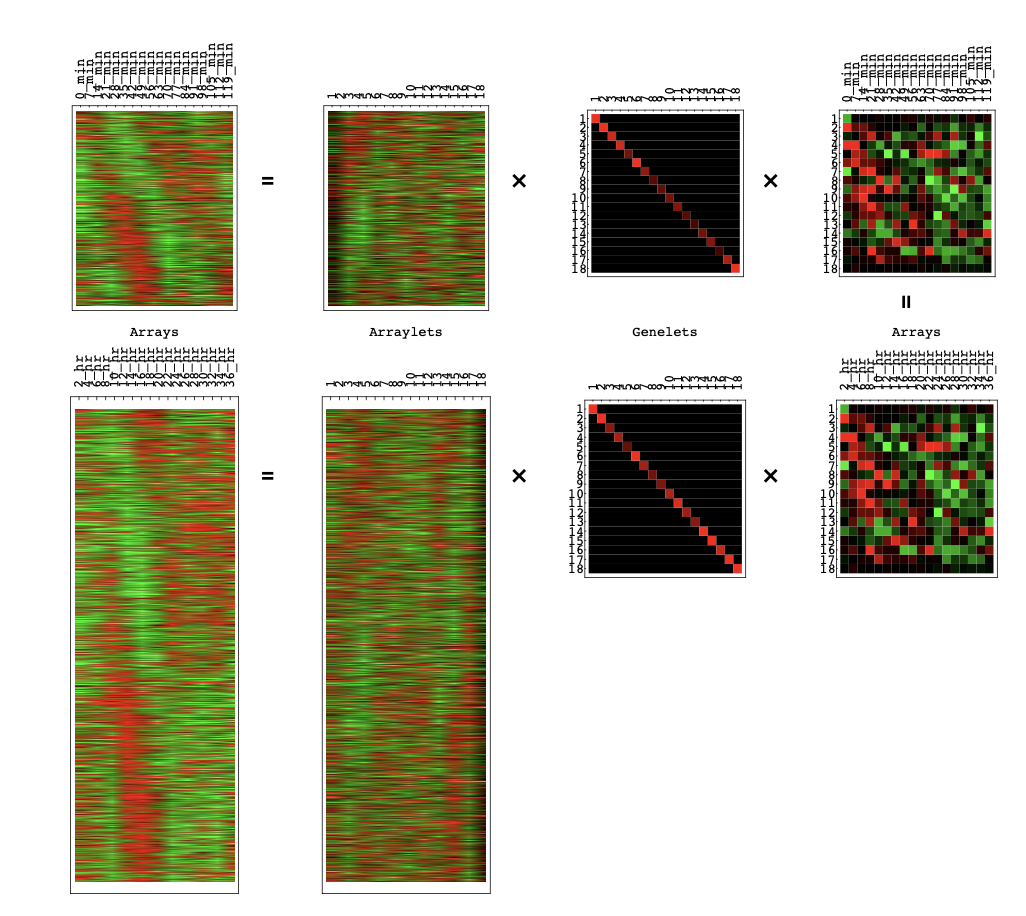
\includegraphics[width=0.85\linewidth]{fig/example_heatmap.png}
        \caption{GSVD of the yeast and human cell-cycle expression data sets. Shown is a heatmap with overexpression (red), no change in expression (black), and underexpression (green)}
        \label{heatmap}
    \end{figure}
    
    We then compute the antisymmetric angular distance defined by \eqref{eq-angular}. By the bar chart of the angular distance, we know that the first and second genlets are highly significant in the yeast data relative to the human data. The third, fourth, and fifth genelets are almost equally significant in both data sets (slightly more in the yeast data), with $0 < \theta_{3}, \theta_{4}, \theta_{}{5} < \pi/16$. The 14th, 15th, and 16th genelets, which are also almost equally significant in both data sets (slightly more in the human data), with $\pi/6 < \theta_{14}, \theta_{15}, \theta_{16} < 0$. The 17th and 18th genelets are highly significant in the human data relative to the yeast data. All other genelets are significant in neither the yeast data nor the human data.
    
    \begin{figure}[H]
        \centering
        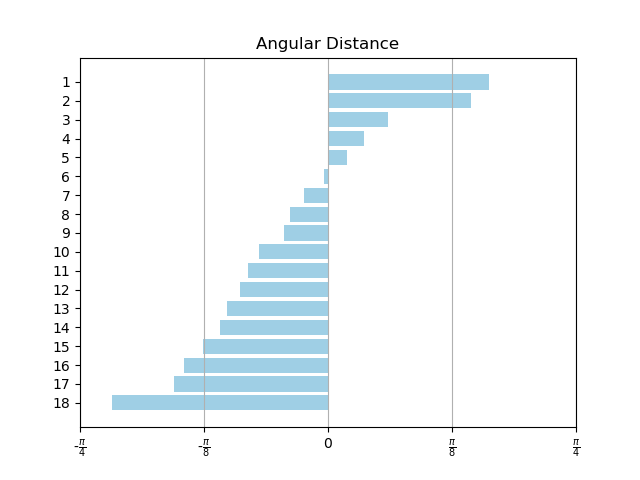
\includegraphics[width=0.5\linewidth]{fig/angulardist.png}
        \caption{Bar chart of the angular distances}
        \label{angulardistance}
    \end{figure}

The GSVD provides a natural solution by creating a single coherent model from the two datasets recording different aspects of interrelated phenomena by simultaneously identifying the similar and dissimilar between the two corresponding column-matched but row-independent matrices. More recently, research conducted by Alter's lab at the University of Utah dive the GSVD into tensor level \cite{bradley2019gsvd} and apply it to the study of tumor, e.g. glioblastoma. \cite{ponnapalli2020retrospective}











